%%%%%%%%%%%%%%%%%%%%%%%%%%%%%%%%%%%%%%%%%%%%%%%%%%%%%%%%%%%%%%%%%%%%%%%%%%%%%%%%
%2345678901234567890123456789012345678901234567890123456789012345678901234567890
%        1         2         3         4         5         6         7         8

\documentclass[letterpaper, 10 pt, conference]{ieeeconf}  % Comment this line out if you need a4paper

%\documentclass[a4paper, 10pt, conference]{ieeeconf}      % Use this line for a4 paper

\IEEEoverridecommandlockouts                              % This command is only needed if 
                                                          % you want to use the \thanks command

\overrideIEEEmargins                                      % Needed to meet printer requirements.

%In case you encounter the following error:
%Error 1010 The PDF file may be corrupt (unable to open PDF file) OR
%Error 1000 An error occurred while parsing a contents stream. Unable to analyze the PDF file.
%This is a known problem with pdfLaTeX conversion filter. The file cannot be opened with acrobat reader
%Please use one of the alternatives below to circumvent this error by uncommenting one or the other
%\pdfobjcompresslevel=0
%\pdfminorversion=4

% See the \addtolength command later in the file to balance the column lengths
% on the last page of the document

% The following packages can be found on http:\\www.ctan.org
\usepackage{graphics} % for pdf, bitmapped graphics files
\usepackage{epsfig} % for postscript graphics files
\usepackage{mathptmx} % assumes new font selection scheme installed
\usepackage{times} % assumes new font selection scheme installed
\usepackage{amsmath} % assumes amsmath package installed
\usepackage{amssymb}  % assumes amsmath package installed
\usepackage{mathtools}
\usepackage{relsize}
\usepackage{tikz}
\graphicspath{{./Drawings/}} 
\newcommand{\notimplies}{%
	\mathrel{{\ooalign{\hidewidth$\not\phantom{=}$\hidewidth\cr$\implies$}}}}
\usepackage{caption}
\newcommand{\norm}[1]{\left\lVert#1\right\rVert}
\usepackage{pgfplots}
\pgfplotsset{compat=newest}
\pgfplotsset{plot coordinates/math parser=false}
\newlength\figureheight
\newlength\figurewidth 

\title{\LARGE \bf
Robust data-driven predictive control
}


\author{Albert Author$^{1}$ and Bernard D. Researcher$^{2}$% <-this % stops a space
\thanks{*This work was not supported by any organization}% <-this % stops a space
\thanks{$^{1}$Albert Author is with Faculty of Electrical Engineering, Mathematics and Computer Science,
        University of Twente, 7500 AE Enschede, The Netherlands
        {\tt\small albert.author@papercept.net}}%
\thanks{$^{2}$Bernard D. Researcheris with the Department of Electrical Engineering, Wright State University,
        Dayton, OH 45435, USA
        {\tt\small b.d.researcher@ieee.org}}%
}


\begin{document}



\maketitle
\thispagestyle{empty}
\pagestyle{empty}


%%%%%%%%%%%%%%%%%%%%%%%%%%%%%%%%%%%%%%%%%%%%%%%%%%%%%%%%%%%%%%%%%%%%%%%%%%%%%%%%
\begin{abstract}

This is a very skeletal overview.

\end{abstract}


%%%%%%%%%%%%%%%%%%%%%%%%%%%%%%%%%%%%%%%%%%%%%%%%%%%%%%%%%%%%%%%%%%%%%%%%%%%%%%%%
\section{Problem Setup}
Consider a \textit{single-input single-output} system $\mathbb{G}_P$ generating an output signal $y(t) \in \mathbb{R}$ corresponding to the input signal $u(t) \in \mathbb{R}$ for the time $t \in \mathbb{Z}$. Consider the data $D_{N}=\{u(t),y(t);t\in{1,...,N}\}$ obtained by exciting the system. 
\\
A feedback controller is designed to control the system, using the VRFT methodology. For this, a reference model $\mathbb{M}_P$ is selected. The VRFT methodology designs a feedback controller  $\mathbb{K}_P$, with the goal of making the closed-loop system $\mathbb{K}_P$-$\mathbb{G}_P$ behave similar to the reference model $\mathbb{M}_P$. To this end, the VRFT methodology utilizes the dataset $\mathbb{D}_N$. The desired closed-loop behavior is described by the LTI state-space model $\mathbb{M}_P$ 

	\begin{equation*}
	\begin{matrix}
	x_M(t+1) = A_Mx_M(t) + B_Mg(t)\\
	y_d(t) = C_Mx_M(t)
	\end{matrix}
	\end{equation*}\\    
The VRFT methodology utilized to design the feedback controller $\mathbb{K}_P$ is now explained:
\begin{enumerate}
	\item
	A virtual reference input $g(t)$ is calculated by setting $y_d(t)=y(t)$ obtained from the dataset $\mathbb{D}_N$, by the inverting the model $\mathbb{M}_P$. Let this mapping be defined by $g(t) = \mathbb{M}_P^{\dagger}y(t) $.
	\item
	A feedback controller $\mathbb{K}_P$ described by $A_K(q^{-1})u(t) = B_K(q^{-1})(g(t)-y(t)$ is chosen, where 
	\begin{equation*}
	\begin{matrix}
	A_K(q^{-1}) = 1+\mathlarger{\sum\limits_{i=1}^{n_{a_K}}}a_i^Kq^{-i}\\
	B_K(q^{-1}) = \mathlarger{\sum\limits_{i=1}^{n_{b_K}}}b_i^Kq^{-i}
	\end{matrix}  
	\end{equation*}
	The parameters of the controller $a_i^K$ and $b_i^K$ are calculated by the VRFT methodology, such that the closed loop performance of $\mathbb{K}_P$-$\mathbb{G}_P$ matches open loop performance of  the reference model $\mathbb{M}_P$.
	\item
	This is done by solving the convex optimization problem
	\begin{equation*}
	\begin{aligned}
	& \underset{a_i^K,b_i^K}{\text{min}}
	& & \frac{1}{N}\mathlarger{\sum\limits_{t=1}^N}\mathlarger{\mathlarger{|}}A_K(q^{-1})u(t)-B_K(q^{-1})(\mathbb{M}_P^{\dagger}y(t)-y(t))\mathlarger{\mathlarger{|}}^2 \\
	\end{aligned}
	\end{equation*}
	which minimizes the deviation between the control input calculated by the controller and $u(t)$ that is used to excite the system and obtain $y(t)$.
	\item
	The synthesized controller $\mathbb{K}_P$ is placed before the plant, and the loop is closed. A reference step input is given to evaluate the controller performance.
	\begin{figure}[h]
	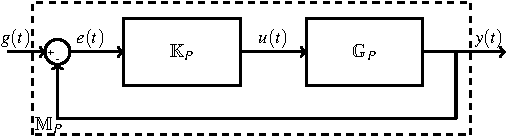
\includegraphics{KpGp.pdf}
	\end{figure}
	\\
	The performance of this setup is improved by providing the reference signal $g(t)$ using an MPC controller in an outer loop. The objective of the MPC controller is to make the output signal $y(t)$ track the reference $r(t)$, while satisfying constraints on the plant output $y(t)$ and input $u(t)$. This is achieved by considering the closed-loop plant model $\mathbb{M}_P$ for the state propagation equation, and an augmented model with $[y(t),u(t)]$ as the output equation. This augmented state-space model is called $\mathbb{M}'_P$.
	\begin{equation*}
	\begin{matrix}
	\zeta(t+1) = A_\zeta\zeta(t) + B_\zeta g(t)\\
	\begin{bmatrix}y(t)\\u(t)\end{bmatrix} = C_\zeta\zeta(t) + D_\zeta g(t)
	\end{matrix}
	\end{equation*}
	\\
	The optimization problem solved by the MPC at each time step $t$ for a horizon of $N_P$ timesteps is shown below. The lower and upper bounds on $y(t)$ and $u(t)$ are $[y_{min},y_{max}]$ and $[u_{min},u_{max}]$ respectively.
	\begin{equation}
	\begin{aligned}
	& \underset{\{g(t+k)\}_{k=1}^{N_P}}{\text{min}}
	& & Q_y\mathlarger{\sum\limits_{k=1}^{N_P}}(y(t+k|t)-r(t+k))^2 + Q_{\epsilon}\epsilon^2 \\
	& \text{subject to}
	& & 
	\begin{matrix}
	\zeta(t+k+1) = A_\zeta\zeta(t+k) + B_\zeta g(t+k)\\
	\begin{bmatrix}y(t+k)\\u(t+k)\end{bmatrix} = C_\zeta\zeta(t+k) + \begin{bmatrix}0\\D_\zeta\end{bmatrix}g(t+k)\\
	y_{min}-V_y\epsilon \leq y(t+k) \leq y_{max}+V_y\epsilon \\
	u_{min}-V_u\epsilon \leq u(t+k) \leq u_{max}+V_u\epsilon \\
	\zeta(t|t) = \zeta(t)
	\end{matrix}
	\end{aligned}
	\label{MPC}
	\end{equation}
	\\
	The quantities $V_y$ and $V_u$ in the MPC formulation are used to avoid infeasibility of the optimization problem over successive iterations, since the reference model $\mathbb{M}'_P$ might not accurately capture the dynamics of the unknown plant $\mathbb{G}_P$. This implies that constraint satisfaction is not guaranteed by the proposed formulation. 
	
	\section{Disturbance sensor}
	In order to improve prediction of closed loop performance, a disturbance sensor $\mathbb{D}$ is designed. The disturbance sensor is a dynamical system whose output is the discrepancy between output of the actual closed loop system  $\mathbb{K}_P$-$\mathbb{G}_P$ and reference closed loop system $\mathbb{M}_P$. The system consists of a deterministic part and a stochastic part, as seen in Fig. \ref{Appended}.
	\begin{figure}[h]
		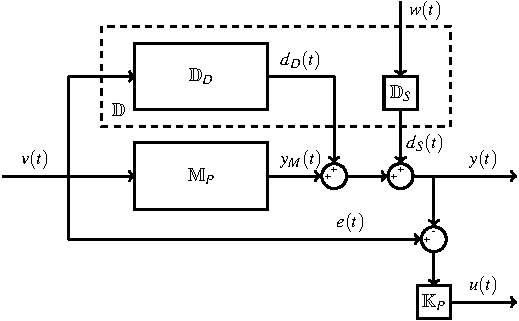
\includegraphics{Mp-D-E.pdf}
		\caption{Reference model appended with disturbance sensor}
		\label{Appended}
	\end{figure}
	\\
	This can be seen as a 2-input 2-output system, whose transfer function is described as
	\begin{equation}
	\begin{bmatrix}
		Y(z) \\ U(z)
	 \end{bmatrix} = 
	 \begin{bmatrix} 
	 \mathbb{M}_P+\mathbb{D}_D & \mathbb{D}_S \\
	 \mathbb{K}_P(I-(\mathbb{M}_P+\mathbb{D}_D)) &  -\mathbb{K}_P\mathbb{D}_S
	 \end{bmatrix}
	 \begin{bmatrix}
	 G(z) \\ W(z)
	 \end{bmatrix}
	 \label{TF}
	\end{equation}
	Note that the dependence of transfer functions on time shift operator $z$ (or $q^{-1}$) is not denoted for ease of notation. The signal $w(t)$ is interpreted as an external noise signal. 
	Since this model represents the closed loop behavior of the system, new closed loop measurements are required to estimate the parameters of the disturbance sensor. These are obtained by performing experiments with excitaion signals $\hat{g}(t)$ on the closed loop model and plant, and measuring the outputs $\hat{y}_M(t)$ and $\hat{y}(t)$ respectively. The output is captured as the data sequence $\hat{D}_{N}=\{\hat{g}(t),\hat{y}_M(t),\hat{y}(t);t\in{1,...,N}\}$.
	The disturbance sensor $\mathbb{D}$ is parameterized as $A_D(q^{-1})y_D(t) = B_D(q^{-1})g(t)+w(t)$, where 
	\begin{equation*}
	\begin{matrix}
	y_D(t) = y(t) - y_M(t) = d_D(t)+d_S(t) \\ 
	A_D(q^{-1}) = 1+\mathlarger{\sum\limits_{i=1}^{n_{a_D}}}a_i^Dq^{-i}\\
	B_D(q^{-1}) = \mathlarger{\sum\limits_{i=1}^{n_{b_D}}}b_i^Dq^{-i}
	\end{matrix}  
	\end{equation*}
	Using standard ARX identification, the coefficients $a_i^D$ and $b_i^D$ are estimated by solving the optimization problem
	\begin{equation*}
	\begin{aligned}
	& \underset{a_i^D,b_i^D}{\text{min}}
	& & \frac{1}{N}\mathlarger{\sum\limits_{t=1}^N}\mathlarger{\mathlarger{|}}A_D(q^{-1})(\hat{y}(t)-\hat{y}_M(t))-B_K(q^{-1})(\hat{g}(t))\mathlarger{\mathlarger{|}}^2 \\
	\end{aligned}
	\end{equation*}
	The disturbance sensor is then split into two parts, deterministic and stochastic. The deterministic part $\mathbb{D}_D$ takes in the reference signal $g(t)$ as an input, and the stochastic part $\mathbb{D}_S$ takes in the noise $w(t)$. The I/O behavior of these parts are separately written as 
	\begin{equation*}
	\begin{matrix}
	d_D(t) = \cfrac{B_D(q^{-1})}{A_D(q^{-1})}g(t) = \mathbb{D}_D g(t) \vspace{4pt} \\  
	d_S(t) = \cfrac{1}{A_D(q^{-1})}w(t) = \mathbb{D}_S w(t)
	\end{matrix}
	\end{equation*}
	Once all the parameters of the disturbance sensor are calculated, the model \eqref{TF} can be used in a formulation similar to \eqref{MPC} to generate optimal input signal $g(t)$. However, the model has an additional noisy input $w(t)$, which will be transformed to process and measurement noises on the state space model corresponding to \eqref{TF}. Hence, it is desirable to calculate upper and lower bounds $w_{min}$ and $w_{max}$ on the noise signal $w(t)$, and explicitly provide them to the optimization problem in order to obtain as robust formulation.\\
	\section{Noise input bounds calculation}
	\label{Noise}
	A realization of the discrepancy $d_S(t)$ between desired output $y(t)$ and deterministic output $y_M(t)+d_D(t)$ can be calculated from the data set $\hat{D}_{N}$ as 
	\begin{equation*}
	\hat{d}_S(t) = \hat{y}(t)-\hat{y}_M(t)-\cfrac{B_D(q^{-1})}{A_D(q^{-1})} \hat{g}(t) 
	\end{equation*}
	The maximum and minimum values of this discrepancy are labeled $\hat{d}_{S,max}$ and $\hat{d}_{S,min}$ respectively. If the ARX estimation results in a stable deterministic disturbance sensor $\mathbb{D}_D$, the values $\hat{d}_{S,max}$ and $\hat{d}_{S,min}$ are finite. Further, if infinite closed loop data $\hat{D}_{\infty}$ is collected for ARX estimation, the bounds on discrepancy are equal to the actual bounds $d_{D,max}$ and $d_{D,min}$. The set of sequences $d_S(t)$ satisfying these bounds are indicated as lying in a set $D_{\infty}$, defined as 
	\begin{equation*}
	D_{\infty} = \{d_S(t): d_{S,min} \leq d_S(t) \leq d_{S,max} \hspace{5pt} \forall t \in (-\infty,\infty) \}
	\end{equation*}
	 From these bounds, we attempt to calculate the set $W_{\infty}$ defined as
	\begin{equation*}
	W_{\infty} = \begin{Bmatrix} w(t): \forall t \in (-\infty,\infty), \begin{matrix}
	w_{min}\leq w(t)\leq w_{max} \\ 
	\mathbb{D}_S w(t) \in D_{\infty} \\
	\end{matrix} 
	\end{Bmatrix}
	\end{equation*}  
	This is the set of all $w(t)$ sequences such that the output signal of $\mathbb{D}_S$ corresponding to any $w(t)\in W_{\infty}$  lies within the bounds $[d_{S,min},d_{S,max}]$. It must be noted that the converse is not implied. That is, it does not mean that there cannot exist a noise sequence $w(t)$ not belonging to $W_{\infty}$ but producing a corresponding output sequence belonging to $D_{\infty}$.
	\begin{equation*}
	\forall w(t) \in W_{\infty}  : \mathbb{D}_S w(t) \in D_{\infty} \notimplies \nexists  w(t) \notin W_{\infty} : \mathbb{D}_S w(t) \in D_{\infty}
	\end{equation*}
	To calculate the bounds $w_{min}$ and $w_{max}$, the optimization problems shown in \ref{bounds} are solved for increasing lengths of time horizon $N$.
	\begin{figure*}[h]
	\begin{center}
	\begin{tabular}[h]{c|c}
		\centering
		\setlength{\tabcolsep}{0.1em}
		$
		\begin{matrix}
		\underset{X_{min}}{\text{max}}
		& w^N_{min} \\
		\text{subject to}
		& 
		d_S(k) = -\mathlarger{\sum\limits_{i=1}^{n_{a_D}}}a_i^Dd_S(k-i) + w(k), k={1:N}\\
		& d_{S,min} \leq d_S(k) \leq d_{S,min}, k={1:N-1} \vspace{4pt}\\
		& w^N_{min} \leq w(k), k={1:N} \vspace{3pt}\\
		& d_S(N) \leq d_{S,min} 
		\end{matrix} 
		$
		&
		$
		\begin{matrix}
			\underset{X_{max}}{\text{min}}
			& w^N_{max} \\
			\text{subject to}
			&
			d_S(k) = -\mathlarger{\sum\limits_{i=1}^{n_{a_D}}}a_i^Dd_S(k-i) + w(k), k={1:N}\\
			& d_{S,min} \leq d_S(k) \leq d_{S,min}, k={1:N-1} \vspace{4pt}\\
			& w(k) \leq w^N_{max}, k={1:N} \vspace{3pt}\\
			& d_S(N) \geq d_{S,max} \\
		\end{matrix}
		$
		\vspace{10pt}\\
		$
		\text{where } X_{min} = 
		\begin{Bmatrix}
		\{d_S(-n_{a_D}+1),...,d_S(N)\},\\
		\{w(1),...,w(N)\},\vspace{0.001cm}\\
		w^N_{min}
		\end{Bmatrix}
		$
		&
		$
			\text{where } X_{max} = 
			\begin{Bmatrix}
			\{d_S(-n_{a_D}+1),...,d_S(N)\},\\
			\{w(1),...,w(N)\},\vspace{0.001cm}\\
			w^N_{max}
			\end{Bmatrix}
			$
	\end{tabular}
	\end{center}\mbox{} 
	\label{bounds}
	\caption{Linear programs solved to calculate the set $W_{\infty}$}
	\end{figure*}
	These equations solve for a sequence of inputs $\{w(k), k={1:N}\}$ such that the sequence of corresponding outputs at all instances except at time $N$ lie within $D_{\infty}$. This means that the chosen input sequence $w(k)$ can drive the system output out of bounds in $N$ time steps. The initial conditions on $d_S(k)$ are left free to be chosen by the problem, but are constrained to lie within $D_{\infty}$. Thus, for a time horizon $N$, the input $\{w(k), k={1:N}\}$ is chosen such that, wherever the system starts inside the set $D_{\infty}$, it will stay inside the set $D_{\infty}$. This freedom to choose an initial condition also permits the assumption that $D_{\infty}$ is obtained from the infinite data set $\hat{D}_{\infty}$.
	\\
	\noindent
	Any sequence $\{w(k)>w^N_{min},k=1:N\}$ will not drive $d_S(k \geq N)$ to the bound $d_{S,min}$. Similarly, $\{w(k)<w^N_{max},k=1:N\}$ will not drive $d_S(k \geq N)$ to the bound $d_{S,max}$. Hence, in order to explain the whole set $D_{\infty}$, we need to find the lowest possible value of $w^N_{min}$ and the highest possible value of $w^N_{max}$ such that $d_S(k)$ is driven to its bounds in finite time $k$. This is achieved by increasing the value of $N$, which would require lower and higher values of $w(k)$ to make $d_S(N)$ reach $d_{S,min}$ and $d_{S,max}$ respectively. This leads to $w^N_{min}$ and $w^N_{max}$ asymptotically reaching their true values $w_{min}$ and $w_{max}$ as $N$ increases, thus making the set $W_{\infty}$ completely explain the set $D_{\infty}$. It is noted that the presented method provides a methodology to quantify uncertainty in any general ARX identified model.
	\\
	After finding bounds on the noise, the appended model with disturbance sensor can be used in a robust control framework. In the current work, a robust reference governer is developed. The reference governer alters the reference input $g(t)$ from the MPC algorithm in \eqref{MPC} to generate a new reference signal $v(t)$, for which the closed loop plant satisfies output constraints.
	\section{Robust reference governer}
	The robust reference governer is a signal regulator which alters the command input such that the system robustly satisfies constraints. It does so by utilizing knowledge of disturbances acting on the system. A schematic of the control system is shown in Fig. \ref{fullloop}. 
	\begin{figure}[h]
		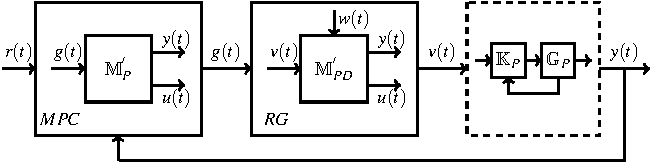
\includegraphics[scale = 0.8]{withRG.pdf}
		\caption{Schematic of the control system}
		\label{fullloop}
	\end{figure} \\
	The $MPC$ controller utilizes the model $\mathbb{M}'_{P}$, and the reference governer $RG$ uses the model $\mathbb{M}'_{PD}$, which is the state space representation of \eqref{TF}. This is written as:
	\begin{equation*}
	\begin{matrix}
	\gamma(t+1) = A_\gamma\gamma(t) + B^v_\gamma v(t) + B^w_\gamma w(t) \vspace{2pt}\\
	\begin{bmatrix}y(t)\\u(t)\end{bmatrix} = C_\gamma\gamma(t) + D^v_\gamma v(t) + D^w_\gamma w(t)
	\end{matrix}
	\end{equation*}
	The columns of matrices $B_\gamma$ and $D_\gamma$ are separated for ease of notation. The outputs of the system are called $y_{\gamma}(t)=[y(t) u(t)]^T$. The constraints on these outputs are written as: 
	\begin{equation*}
	\begin{matrix}
	\begin{matrix}
	y_{min} \leq y(t) \leq y_{max} \\
	u_{min} \leq u(t) \leq u_{max}
	\end{matrix} & \bigg{\}} & Hy_{\gamma}(t) \leq h
	\end{matrix}
	\end{equation*}
	At each time instant $t$, the reference governer solves the quadratic program:
	\begin{equation}
	\begin{aligned}
	& \underset{v}{\text{min}}
	& & \cfrac{1}{2}\norm{v-g(t)}_2^2 \\
	& \text{subject to}
	& & 
	(x(t),v) \in \mathbb{O}_{\infty}
	\end{aligned}
	\label{RGprob}
	\end{equation}
	where the set $\mathbb{O}_{\infty}$ is defined as:
	\begin{equation*}
	\mathbb{O}_{\infty} = \{(x(t),v): x(t) = \gamma(t), \hspace{2pt} Hy_{\gamma}(\tau) \leq h \hspace{5pt} \forall \tau \geq t \} \\ 
	\end{equation*}
	This is called an output-invariant set.
	It is set of feasible values for $v$ for the current observed state $x(t)=\gamma(t)$ such that if a constant input signal $v(\tau \geq t)=v$ is applied, the system output constraints $Hy_{\gamma}(\tau \geq t) \leq h$ remain satisfied for all $\tau$.
	At a time instant $\tau \geq t$, the system output $y_{\gamma}(\tau)$ for input signal $v(\tau \geq t)=v$ can be written as:
	\begin{equation*}
	\hspace{-30pt}
	\begin{aligned}
	\begin{matrix}
	y_{\gamma}(\tau) = C_{\gamma}A_{\gamma}^{\tau - t}\gamma(t) + \bigg( C_{\gamma}\sum\limits_{k=1}^{\tau - t}A_{\gamma}^{k-1}B^v_{\gamma} + D_{\gamma}^v \bigg)v + \vspace{5pt}\\  \hspace{110pt} C_{\gamma}\sum\limits_{k=1}^{\tau - t}A_{\gamma}^{k-1}B^w_{\gamma}w(\tau-k) + D_{\gamma}^w w(\tau)
	\end{matrix}
	\end{aligned}
	\end{equation*} \vspace{24pt}\\
	For a particular future time instant $\tau$, the set $\mathbb{O}_{\infty}(\tau)$ is given by:
	\begin{equation*}
	\begin{matrix}
	\mathbb{O}_{\infty}(\tau) = \{(x(t),v): x(t) = \gamma(t), \hspace{5pt} \tilde{H}(\tau)v \leq \tilde{h}(\tau)\} \vspace{5pt}\\
	\text{where } \hspace{5pt} \tilde{H}(\tau) = H\bigg( C_{\gamma}\sum\limits_{k=1}^{\tau - t}A_{\gamma}^{k-1}B^v_{\gamma} + D_{\gamma}^v \bigg) \vspace{5pt} \\ \hspace{10pt}
	\tilde{h}(\tau) = h - HC_{\gamma}A_{\gamma}^{\tau - t}\gamma(t) - f^w(\tau) \vspace{5pt}
	\end{matrix} 
	\end{equation*}
	Each element $f^w_i(\tau)$ of the column vector $f^w(\tau)$ is calculated by solving the linear program:
	\begin{equation*}
	f_i^w(\tau) = \underset{\{w(k)\}_{t}^{\tau}\in W_{\infty}}{\text{max}} H\bigg(C_{\gamma}\sum\limits_{k=1}^{\tau - t}A_{\gamma}^{k-1}B^w_{\gamma}w(\tau-k) + D_{\gamma}^w w(\tau)\bigg)_i
	\end{equation*}
	Subscript $i$ in the above problem indicates that row $i$ of the matrix is used in the linear program to calculate the corresponding $w(k)$ sequence. According to the theory of output invariant sets for linear systems with polyhedral constraints on noise and outputs, the set $\mathbb{O}_{\infty} = \mathbb{O}_{\infty}(\tau \to \infty)$ is reached when the elements of $f^w(\tau)$ converge to a constant value. Since the linear problem to be solved for $f_i^w(\tau)$ does not depend on values at current time instant $t$, it can be solved offline for increasing values of $\tau$. When convergence is observed at time $\tau_c$, the value $f^w(\tau_c)$ is stored. This results in  problem \eqref{RGprob} being simplified to
	\begin{equation}
	\begin{aligned}
	& \underset{v}{\text{min}}
	& & \cfrac{1}{2}\norm{v-g(t)}_2^2 \\
	& \text{subject to}
	& & 
	\tilde{H}(\tau_c)v \leq \tilde{h}(\tau_c)
	\end{aligned}
	\label{RGprob_simple}
	\end{equation}
	It must be noted that the value $\tilde{h}(\tau_c)$ depends on the current observed state $\gamma(t)$. Thus, at each time instant, the reference governer reads the current state $\gamma(t)$, reference input $g(t)$, and calculates a new reference $v(t)$ which satisfies output constraints on the system robustly.
	\section{Case studies}
	\subsection{Noise input bound}
	Consider a MISO system with inputs $\{u(t),w(t)\}$ and output $x(t)$, described by:
	\begin{equation*}
	\begin{matrix}
	u(t+1) = 0.995u(t)+1 \\
	x(t+1) = 0.05x(t)+u(t)+w(t) \\
	u(1) = 0, \hspace{5pt} x(1) = 0
	\end{matrix}
	\end{equation*}
	The input $u(t)$ is deterministic and $w(t)$ is noisy. An approximate ARX model of the system is calculated as $A(q^{-1})\tilde{x}(t) = B(q^{-1})u(t)+w(t)$ after performing experiments on the system and collecting data. It is identified with $A(q^{-1})$ and $B(q^{-1})$ having 2 and 1 free parameters respectively. Following this, the methodology discussed in Sec.\ref{Noise} is used to calculate bounds on $w(t)$.
	\\
	First, the signal $d_S(t)=x(t) - (B(q^{-1})/A(q^{-1}))u(t)$ is extracted from the experimental data, and $D_{\infty}$ is constructed. For increasing values of $N$, sequences $\{w(k),k=1:N\}$ and corresponding $\{d_S(k),k=1:N\}$ are calculated by solving the optimization problems in \ref{bounds}. The bounds $w^N_{min}$ and $w^N_{max}$ on the input sequences are shown in Fig.\ref{bounds}.
	\begin{figure}[h]
		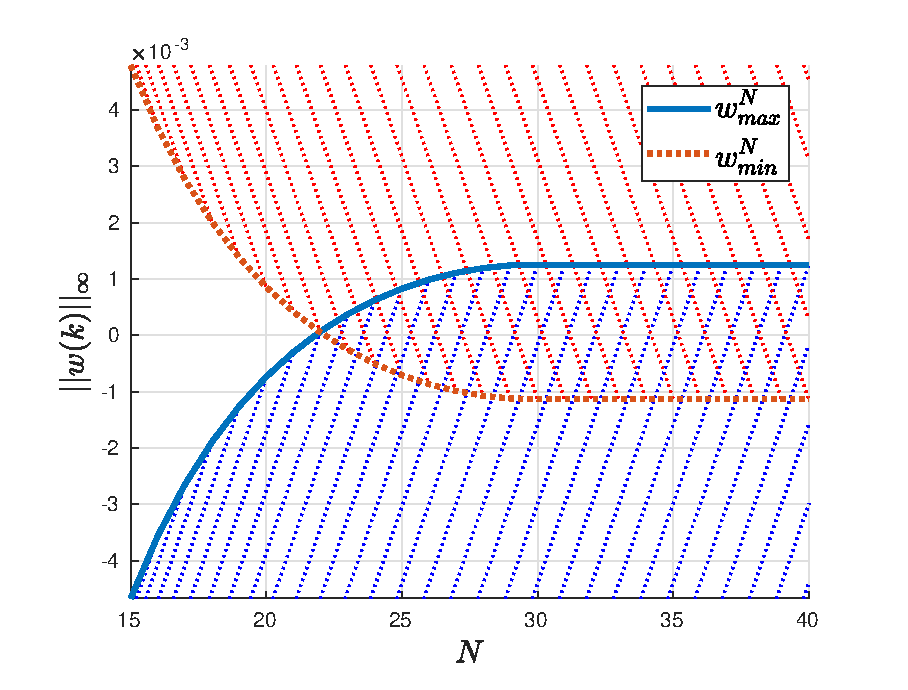
\includegraphics[scale = 0.55]{bounds.eps}
		\caption{Convergence of bounds to $w_{min}$ and $w_{max}$}
		\label{bounds}
	\end{figure} 
	The largest region where $w^N_{min} \leq w(k) \leq w^N_{max}$ is satisfied is $W_{\infty}$. To verify the obtained bounds, the system identified through ARX identification is simulated with deterministic inputs $u(t)$, and a range of noise inputs $w(t)$ sampled from $W_{\infty}$ and held constant throughout the simulation horizon. The simulation results are seen in Fig.\ref{simulation}.
	\begin{figure}[h]
		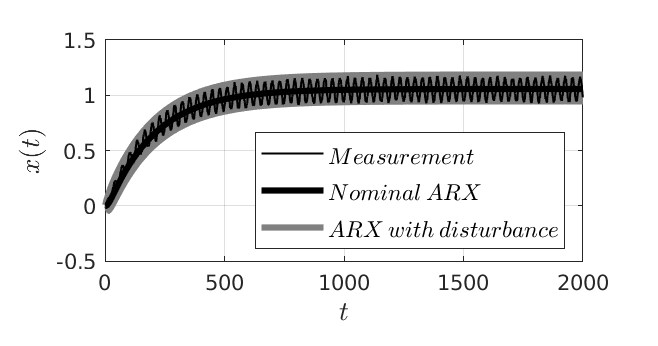
\includegraphics[scale = 0.65]{simulation.eps}
		\caption{Comparison of ARX model performance with constant $w(t)=0$(nominal) and $w(t)\in W_{\infty}$. The noise model gives bounded output $x(t)$ without being conservative.}
		\label{simulation}
	\end{figure} \\
	The simulation of ARX model with noise requires an initial condition on the noise model. However, the problem calculates $W_{\infty}$ for all $D_{\infty}$ without incorporating the knowledge of an initial condition (This is the main feature of the problem). In the current example, the ARX model with noise is simulated with a initial condition = $0$. Since the actual initial condtion of the noise model might not be $0$, one might face problems with the model not covering the whole range of $D_{\infty}$ during the transient period. To correct this, a state estimator could be used which rectifies the effect of initial state discrepancy, thus covering the noise effects even during transients.
	\subsection{Data driven MPC with robust reference governer}
	Simulations are performed on a model of a servo positioning system, controlled using the loop presented in Fig.\ref{fullloop}. The plant dynamics are modeled with the following non-linear state space equations:
	\begin{equation*}
	\begin{matrix}
	\begin{bmatrix}
	\dot{\theta}(t) \vspace{12pt} \\
	\dot{\omega}(t) \vspace{12pt} \\
	\dot{i}(t)
	\end{bmatrix} = 
	\begin{bmatrix}
	\omega(t) \vspace{3pt}\\
	\cfrac{-mgl}{J}\hspace{1pt}sin\theta(t)-\cfrac{b}{J}\hspace{1pt}\omega(t) + \cfrac{K_m}{J}\hspace{1pt}i(t) \\  
	\cfrac{-K_m}{L}\hspace{1pt}\omega(t)-\cfrac{R}{L}\hspace{1pt}i(t) + \cfrac{1}{L}\hspace{1pt}u(t)
	\end{bmatrix} \vspace{10pt}\\
	y(t) = \begin{bmatrix} 1 & 0 & 0 \end{bmatrix} 
	\begin{bmatrix} \theta(t) \\ \omega(t) \\ i(t) \end{bmatrix} 
	\end{matrix}
	\end{equation*}
	
	\begin{center}
		\begin{tabular}{||c|c|c||} 
			\hline
			Symbol & Parameter & Value\\ [0.5ex] 
			\hline\hline
			$R$ & Motor resistance & $5$\Omega\\ 
			\hline
			$L$ & Motor inductance & $5.10^{-3}$H \\
			\hline
			$K_m$ & Motor torque constant & $0.0847$Nm/A \\
			\hline
			$J$ & Complete disk inertia & $5.10^{-5}$Nm^2 \\
			\hline
			$b$ & Friction coefficient & $3.10^{-3}Nms/rad$ \\ [1ex] 
			\hline
		\end{tabular}
	\end{center}
	
	
	
	
	
	
	
\end{enumerate} 

	
                                                              




\begin{thebibliography}{99}

\bibitem{c1} G. O. Young, �Synthetic structure of industrial plastics (Book style with paper title and editor),� 	in Plastics, 2nd ed. vol. 3, J. Peters, Ed.  New York: McGraw-Hill, 1964, pp. 15�64.
\bibitem{c2} W.-K. Chen, Linear Networks and Systems (Book style).	Belmont, CA: Wadsworth, 1993, pp. 123�135.
\bibitem{c3} H. Poor, An Introduction to Signal Detection and Estimation.   New York: Springer-Verlag, 1985, ch. 4.
\bibitem{c4} B. Smith, �An approach to graphs of linear forms (Unpublished work style),� unpublished.
\bibitem{c5} E. H. Miller, �A note on reflector arrays (Periodical style�Accepted for publication),� IEEE Trans. Antennas Propagat., to be publised.
\bibitem{c6} J. Wang, �Fundamentals of erbium-doped fiber amplifiers arrays (Periodical style�Submitted for publication),� IEEE J. Quantum Electron., submitted for publication.
\bibitem{c7} C. J. Kaufman, Rocky Mountain Research Lab., Boulder, CO, private communication, May 1995.
\bibitem{c8} Y. Yorozu, M. Hirano, K. Oka, and Y. Tagawa, �Electron spectroscopy studies on magneto-optical media and plastic substrate interfaces(Translation Journals style),� IEEE Transl. J. Magn.Jpn., vol. 2, Aug. 1987, pp. 740�741 [Dig. 9th Annu. Conf. Magnetics Japan, 1982, p. 301].
\bibitem{c9} M. Young, The Techincal Writers Handbook.  Mill Valley, CA: University Science, 1989.
\bibitem{c10} J. U. Duncombe, �Infrared navigation�Part I: An assessment of feasibility (Periodical style),� IEEE Trans. Electron Devices, vol. ED-11, pp. 34�39, Jan. 1959.
\bibitem{c11} S. Chen, B. Mulgrew, and P. M. Grant, �A clustering technique for digital communications channel equalization using radial basis function networks,� IEEE Trans. Neural Networks, vol. 4, pp. 570�578, July 1993.
\bibitem{c12} R. W. Lucky, �Automatic equalization for digital communication,� Bell Syst. Tech. J., vol. 44, no. 4, pp. 547�588, Apr. 1965.
\bibitem{c13} S. P. Bingulac, �On the compatibility of adaptive controllers (Published Conference Proceedings style),� in Proc. 4th Annu. Allerton Conf. Circuits and Systems Theory, New York, 1994, pp. 8�16.
\bibitem{c14} G. R. Faulhaber, �Design of service systems with priority reservation,� in Conf. Rec. 1995 IEEE Int. Conf. Communications, pp. 3�8.
\bibitem{c15} W. D. Doyle, �Magnetization reversal in films with biaxial anisotropy,� in 1987 Proc. INTERMAG Conf., pp. 2.2-1�2.2-6.
\bibitem{c16} G. W. Juette and L. E. Zeffanella, �Radio noise currents n short sections on bundle conductors (Presented Conference Paper style),� presented at the IEEE Summer power Meeting, Dallas, TX, June 22�27, 1990, Paper 90 SM 690-0 PWRS.
\bibitem{c17} J. G. Kreifeldt, �An analysis of surface-detected EMG as an amplitude-modulated noise,� presented at the 1989 Int. Conf. Medicine and Biological Engineering, Chicago, IL.
\bibitem{c18} J. Williams, �Narrow-band analyzer (Thesis or Dissertation style),� Ph.D. dissertation, Dept. Elect. Eng., Harvard Univ., Cambridge, MA, 1993. 
\bibitem{c19} N. Kawasaki, �Parametric study of thermal and chemical nonequilibrium nozzle flow,� M.S. thesis, Dept. Electron. Eng., Osaka Univ., Osaka, Japan, 1993.
\bibitem{c20} J. P. Wilkinson, �Nonlinear resonant circuit devices (Patent style),� U.S. Patent 3 624 12, July 16, 1990. 






\end{thebibliography}




\end{document}
